\documentclass{standalone}
\usepackage{amstext}
\usepackage{amssymb}
\usepackage{tikz}
\usepackage{amsmath}
\usetikzlibrary{shapes.geometric, arrows, calc, positioning}
\usetikzlibrary{decorations.pathreplacing}

\begin{document}
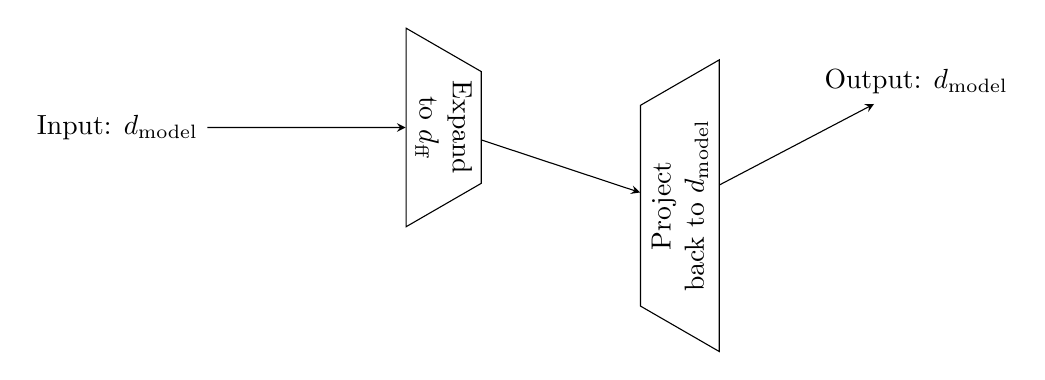
\begin{tikzpicture}[node distance=3cm, auto, >=stealth]

    % Input label (optional)
    \node (input) {Input: $d_{\text{model}}$};

    % Expansion trapezoid: Drawn with a shorter bottom edge and longer top edge.
    % Rotate -90° so the longer edge appears on the right.
    \node[trapezium, 
          trapezium angle=60, 
          draw, 
          rotate=-90, 
          minimum width=2.5cm, 
          %minimum height=1cm, 
          align=center] 
          (expand) [right=of input, anchor=center] {Expand\\to $d_{\text{ff}}$};

    % Projection (contraction) trapezoid: Same shape but rotated 90° to flip the longer edge to the left.
    \node[trapezium, 
          trapezium angle=60, 
          draw, 
          rotate=90, 
          %minimum width=2.5cm, 
          minimum height=1cm, 
          align=center] 
          (contract) [right=of expand, anchor=center] {Project\\back to $d_{\text{model}}$};

    % Output label (optional)
    \node (output) [right=of contract, anchor=center] {Output: $d_{\text{model}}$};

    % Arrows between the nodes
    \draw[->] (input) -- (expand);
    \draw[->] (expand) -- (contract);
    \draw[->] (contract) -- (output);

\end{tikzpicture}
\end{document}

